\documentclass[12pt, a4paper] {ncc}
\usepackage[utf8] {inputenc}
\usepackage[T2A]{fontenc}
\usepackage[english, russian] {babel}
\usepackage[usenames,dvipsnames]{xcolor}
\usepackage{listings,a4wide,longtable,amsmath,amsfonts,graphicx}
\usepackage{indentfirst}
\usepackage{bytefield}
\usepackage{multirow}
\usepackage{float}
\usepackage{caption}
\usepackage{subcaption}
\captionsetup{compatibility=false}
\usepackage{tabularx}

\usepackage[left=2cm,right=2cm,top=2cm,bottom=2cm,bindingoffset=0cm]{geometry}

\begin{document}
\setcounter{figure}{0}
\frenchspacing
\pagestyle{empty}
\begin{center}
                            Университет ИТМО    \\
                        Кафедра вычислительной техники

\vspace{\stretch{2}}
			Основы теории автоматического управления
\end{center}
\vspace{\stretch{2}}
\begin{center}
			Лабораторная работа № 2 \\
		<<Канонические формы представления динамических систем>>
\end{center}
\vspace{\stretch{3}}
\begin{flushright}
                                    Студент:\\
                                    {\it Куклина М.Д., P3401}\\
                                    Преподаватель: \\
                                    {\it Кремлёв А.С.}
\end{flushright}
\vspace{\stretch{4}}
\begin{center}
                             Санкт-Петербург, 2018
\end{center}
\newpage


\section{Аналитический вывод математических моделей канонических форм, подобных систем и матриц преобразования координат}

	\subsection{Переход от модели вход-выход к модели вход-состояние-выход}
		$s^3 y + 2 s^2 y + 5 s y + 7 y = 1.5 s^2 u + 3 s u + 10 u$\\

		$y (s^3 + 2 s^2 + 5 s + 7) = u ( 1.5 s^2 + 3 s + 10)$\\

		Передаточная функция: $W(s) = \dfrac {1.5 s^2 + 3 s + 10} {s^3 + 2 s^2 + 5 s + 7}$

		Таким образом, каноническая управляемая форма:\\
		\begin{center}
    		\[A = 
    			\begin{bmatrix}
    				0 & 1 & 0 \\
    				0 & 0 & 1 \\
    			   -7 & -5 & -2
    			\end{bmatrix}
    		  B = 
				\begin{bmatrix}
					0 \\ 0 \\ 1
				\end{bmatrix}
    		  C = 
				\begin{bmatrix}
					10 & 3 & 1.5
				\end{bmatrix}
			\]
		\end{center}

		Каноническая наблюдаемая форма:\\
		\begin{center}
    		\[A = 
    			\begin{bmatrix}
    				0 & 0 & -7 \\
    				1 & 0 & -5 \\
    			    0 & 1 & -2
    			\end{bmatrix}
    		  B = 
				\begin{bmatrix}
					10 \\ 3 \\ 1.5
				\end{bmatrix}
    		  C = 
				\begin{bmatrix}
					0 & 0 & 1
				\end{bmatrix}
			\]
		\end{center}

	\subsection{Переход от модели вход-состояние-выход к модели вход-выход}

		Исходные данные.
		\begin{center}
    		\[A = 
    			\begin{bmatrix}
    				0.5 & -10 \\
    				1   & -2  \\
    			\end{bmatrix}
    		  B = 
				\begin{bmatrix}
					0 \\ 1 
				\end{bmatrix}
    		  C = 
				\begin{bmatrix}
					3 & 1
				\end{bmatrix}
			\]
		\end{center}

		Передаточная функция:
		$W(S) = C \cdot (s I - A) ^ {-1} \cdot B $\\

		$W(s) = \dfrac {s - 30.5} {s^2 + 1.5 s + 9}$.\\

		Модель вход-выход тогда имеет следующий вид: $y^{(2)} + 1.5 y^{(1)} + 9 y = u ^{(1)} - 30.9 u$.\\

		Из модели вход-выход получаем канонические формы.

		Каноническая управляемая форма:\\
		\begin{center}
    		\[A = 
    			\begin{bmatrix}
    				0  & 1     \\
    				-9 & -1.5  \\
    			\end{bmatrix}
    		  B = 
				\begin{bmatrix}
					0 \\ 1 
				\end{bmatrix}
    		  C = 
				\begin{bmatrix}
					30.9 & 1
				\end{bmatrix}
			\]
		\end{center}

		Каноническая наблюдаемая форма:\\
		\begin{center}
    		\[A = 
    			\begin{bmatrix}
    				0 & -9 \\
    				1 & -1.5 \\
    			\end{bmatrix}
    		  B = 
				\begin{bmatrix}
					30.9 \\ 1
				\end{bmatrix}
    		  C = 
				\begin{bmatrix}
					0 & 1
				\end{bmatrix}
			\]
		\end{center}

	\subsection{Замена базиса в пространстве состояний}
		Исходные данные.
		\begin{center}
    		\[A = 
    			\begin{bmatrix}
    				0.5 & -10 \\
    				1   & -2  \\
    			\end{bmatrix}
    		  B = 
				\begin{bmatrix}
					0 \\ 1 
				\end{bmatrix}
    		  C = 
				\begin{bmatrix}
					3 & 1
				\end{bmatrix}
			  M = 
				\begin{bmatrix}
					4 & 0 \\
					-2 & 0.5 
				\end{bmatrix}
			\]
		\end{center}

		Формулы замены:\\
		$\hat{A} = M^{-1} \cdot A \cdot M$ \\ $\hat{B} = M^{-1} \cdot B$ \\ $ \hat{C} = C \cdot M$. \\

		Результат замены:
		\begin{center}
    		\[A = 
    			\begin{bmatrix}
    				5.5  & -1.25 \\
    				38   & -7  \\
    			\end{bmatrix}
    		  B = 
				\begin{bmatrix}
					0 \\ 2 
				\end{bmatrix}
    		  C = 
				\begin{bmatrix}
					10 & 0.5
				\end{bmatrix}
			\]
		\end{center}
		

\section{Результаты моделирования}

	Результаты моделирования представлены на рисунках 1-6.

	\begin{figure}[ht!]
		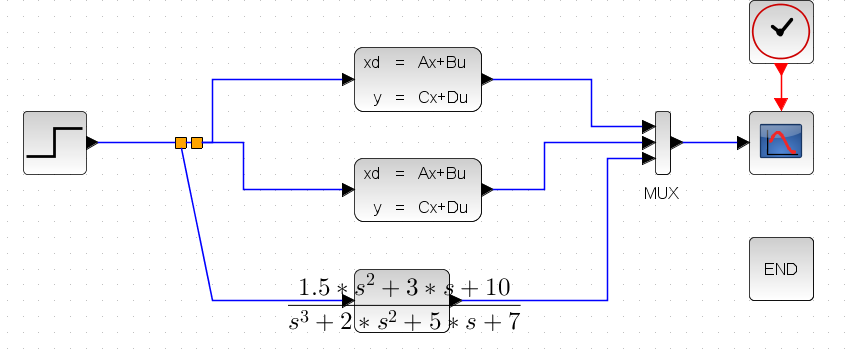
\includegraphics[scale=0.5]{./model1.png}
		\caption{Модель для первого пункта задания.}
	\end{figure}
	\begin{figure}[ht!]
		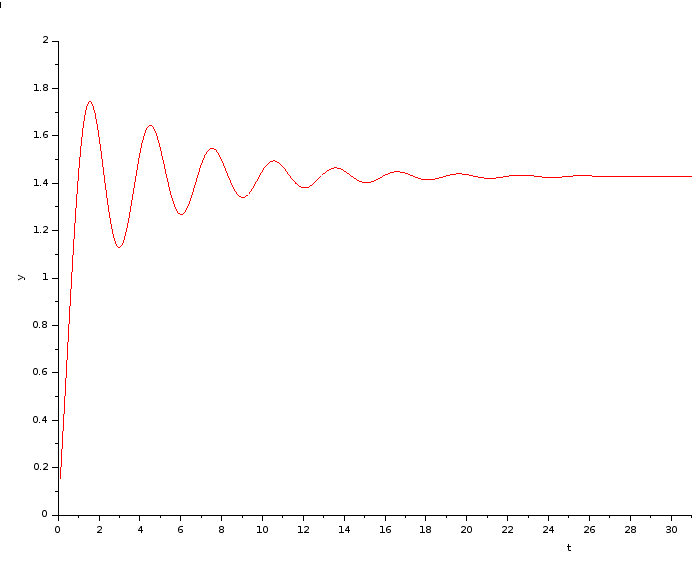
\includegraphics[scale=0.5]{./plot1.png}
		\caption{Результаты моделирования модели вход-выход и модели вход-состояние-выход в каноничных формах
			     при переходе от модели вход-состояние-выход к модели вход-выход.}
	\end{figure}

	\begin{figure}[ht!]
		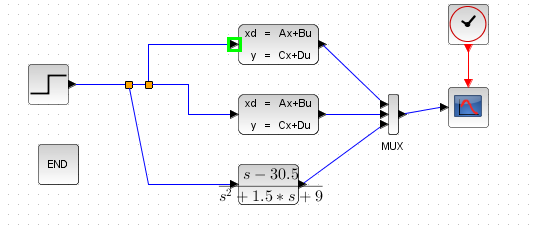
\includegraphics[scale=0.5]{./model2.png}
		\caption{Модель для второго пункта задания.}
	\end{figure}
	\begin{figure}[ht!]
		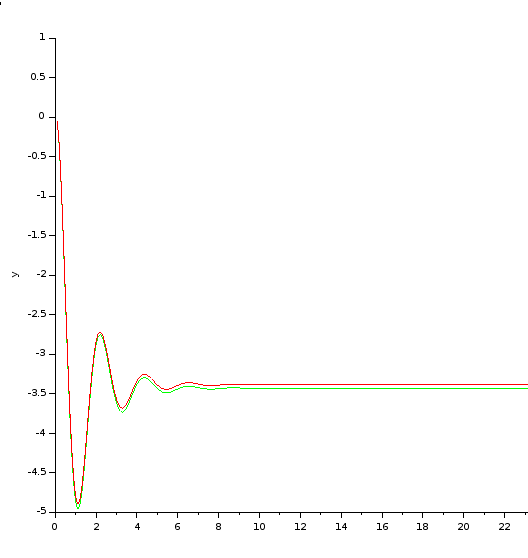
\includegraphics[scale=0.5]{./plot2.png}
		\caption{Результаты моделирования модели вход-выход и модели вход-состояние-выход в каноничных формах
			     при переходе от модели вход-выход к модели вход-состояние-выход.}
	\end{figure}

	\begin{figure}[ht!]
		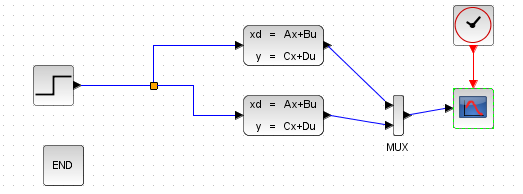
\includegraphics[scale=0.5]{./model3.png}
		\caption{Модель для третьего пункта задания.}
	\end{figure}
	\begin{figure}[ht!]
		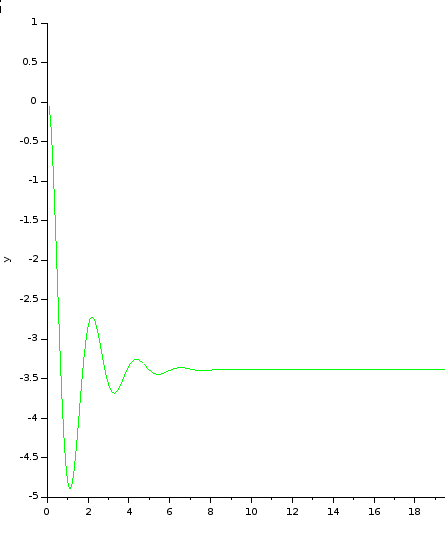
\includegraphics[scale=0.5]{./plot3.png}
		\caption{Результаты моделирования исходной и преобразованной систем}
	\end{figure}



\section{Выводы}

	В результате данной работы я ознакомилась с методами взаимного перехода между моделями
	вход-выход и вход-состояние-вызод, а также с каноническими формами
	представления вход-состояние-выход. В результате моделирования было обнаружено,
	что преобразованные модели идентичны.


\end{document}
